\hspace{24pt}

This paper attempts to improve the zh-ja NMT system by utilizing the phonetic information hidden in the sentences. The complete structure of this paper is shown in Figure~\ref{fig:structure}.

\begin{figure}[h]
	\centering
	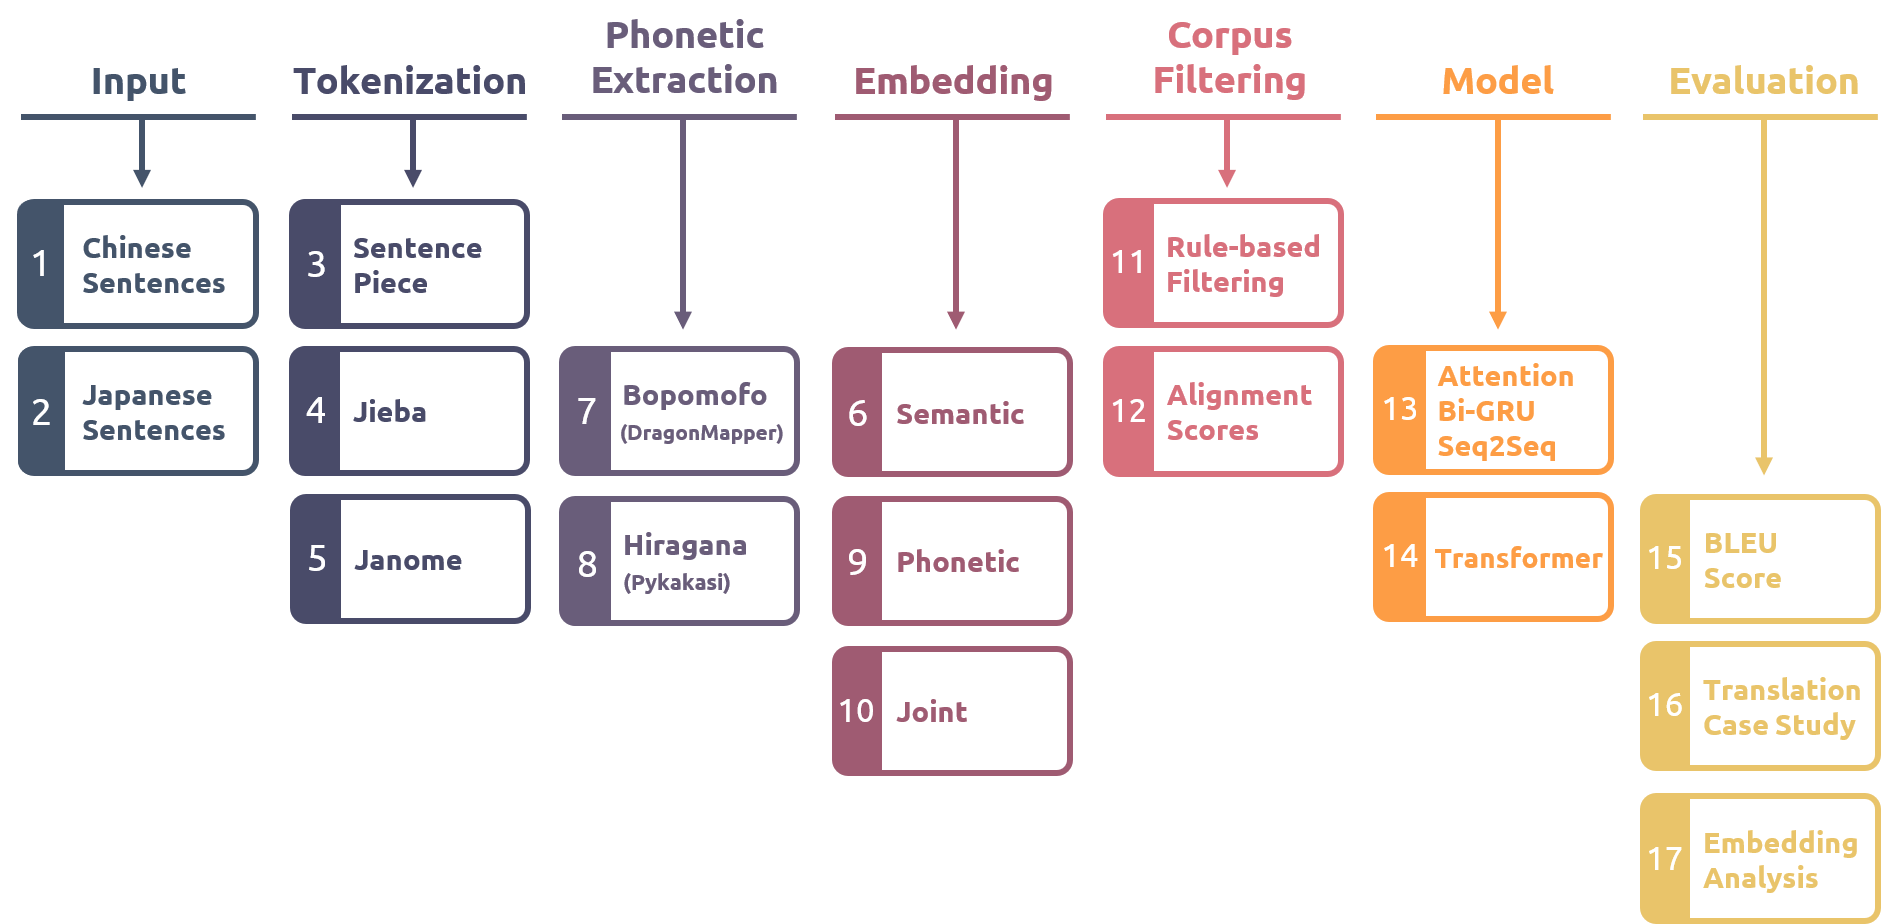
\includegraphics[scale=0.6]{../images/structure.png}
    \caption{The Complete Structure of This Paper}
	\label{fig:structure}
\end{figure}

Section~\ref{sec:tokenization} explains which tokenization methods we use to deconstruct sentences. Section~\ref{sec:phonetic_data} explains which phonetic extraction methods we use to transform plain sentences into phonetic encodings. Section~\ref{sec:embedding} shows how we use Word2Vec as our algorithm to build and combine semantic and phonetic embeddings. Section~\ref{sec:corpus_filtering} shows how we process data from the corpus to eliminate as much noise and reduce the size of the corpus as possible. Section~\ref{sec:nmt_model} explains the details of two NMT models, which are the Attention-based GRU encoder-decoder Model and Transformer. Section~\ref{sec:embedding_analysis} describes the methods we use to analyze the difference between semantic embeddings and joint semantic-phonetic embeddings.

\section{Tokenization} \label{sec:tokenization}

This paper will examine the effectiveness of phonetic information under different tokenization methods. We use the \textit{tokenizers} \footnote{https://github.com/huggingface/tokenizers} library from the \textit{huggingface} team as our main framework for tokenization. SentencePiece \footnote{https://github.com/google/sentencepiece}, Jieba, and Janome can be implemented as pre-tokenizers in Huggingface Tokenizers.

\subsection{Huggingface Tokenizers} \label{sec:tokenizers}

Huggingface Tokenizers has 5 components that allow users to customize their tokenization methods. These five components are normalizers, pre-tokenizers, models, post-processors, and decoders. Normalizers process an input string such as lower cases or remove spaces and symbols to make it normalized. Pre-tokenizers split an input string according to a set of rules, and pre-tokenizers are where we apply SentencePiece, Jieba, and Janome. Models are responsible for converting text into ids by using the rules learned in the corpus (e.g., WordPiece, BPE, Unigram). Post-processors help us to insert special tokens into the sentence, such as the start token \textit{[BOS]} and the end token \text{[EOS]} in NMT tasks. Lastly, the job of Decoders is to reverse the ids to the original sentence.

\subsection{Byte-Pair Encoding (BPE)} \label{sec:bpe}

We use BPE as the model for merging Chinese and Japanese tokens. BPE builds a dictionary of all the words in the corpus and merges the most frequent words to generate new tokens until the maximum number of our dictionary is reached. We demonstrate the basic flow of BPE applied to Chinese through Table \ref{tab:bpe1} and \ref{tab:bpe2}.  

\vspace{0.5cm}
\begin{CJK}{UTF8}{gbsn}
\begin{table}[h]
    \centering
    \begin{tabularx}{.9\textwidth}{sbb}\toprule
        Frequency & Vocabulary & Dictionary \\
        5 & 区\enspace\_ & \_,\enspace区,\enspace地,\enspace经,\enspace济 \\
        7 & 地\enspace区\enspace\_& \\
        3 & 地\enspace区\enspace经\enspace济\enspace\_ & \\
        6 & 经\enspace济\enspace\_ & \\
        \bottomrule
    \end{tabularx}
    \caption{A simple dataset for demonstrating BPE tokenization}
    \label{tab:bpe1}
\end{table}
\end{CJK}

Words are first tokenized by pre-tokenizers and loaded into the BPE vocabulary, with the underscore (\_) representing the end of the words.

\vspace{0.5cm}
\begin{CJK}{UTF8}{gbsn}
    \begin{table}[h]
        \centering
        \begin{tabularx}{.9\textwidth}{ssb}\toprule
            Total Frequency & Merge & New Dictionary \\
            12 & (区,\enspace\_) & \_,\enspace区,\enspace地,\enspace经,\enspace济,\enspace区\_ \\
            9  & (济,\enspace\_) & \_,\enspace区,\enspace地,\enspace经,\enspace济,\enspace区\_,\enspace济\_ \\
            9  & (经,\enspace济\_) & \_,\enspace区,\enspace地,\enspace经,\enspace济,\enspace区\_,\enspace济\_,\enspace经济\_ \\
            7  & (地,\enspace区\_) & \_,\enspace区,\enspace地,\enspace经,\enspace济,\enspace区\_,\enspace济\_,\enspace经济\_,\enspace地区\_ \\
            \bottomrule
        \end{tabularx}
        \caption{The process of merging tokens in BPE tokenization}
        \label{tab:bpe2}
    \end{table}
\end{CJK}

\begin{CJK}{UTF8}{gbsn}
The merge begins with 区 and \_, which appear most frequently in the vocabulary. After merging, 区\_ will be added to the final dictionary and replaces (区\enspace\_) in the vocabulary. This process continues until the final dictionary reaches its maximum size.
\end{CJK}

\subsection{SentencePiece} \label{sec:sentencepiece}

SentencePiece treats all text in the same Unicode format. It will escape the white space with a meta symbol `\_' (U+2581). Therefore, the sentences in Chinese, Japanese, and English are considered to be in the same format, which achieving language independence. 

SentencePiece is a purely data-driven method, which means it relies on the corpus to learn the tokenization. It is simple to implement SentencePiece in Huggingface Tokenizers. First, Normalization Form Compatibility Composition (NFKC) normalizes the sentence, for example, by converting a symbol or text in the full-width form to a normalized form. Second, Metaspace pre-tokenizer splits the sentence by white space and converts the white space into the `\_' symbol. Last, BPE with dropout is applied to train with the corpus file. The dropout method will improve the robustness and accuracy.

\vspace{0.5cm}

\begin{python}
from tokenizers.normalizers import NFKC
from tokenizers import Tokenizer, pre_tokenizers, decoders, trainers

tokenizer = Tokenizer(BPE(dropout=dropout, unk_token="[UNK]"))
tokenizer.normalizer = NFKC()
tokenizer.pre_tokenizer = pre_tokenizers.Metaspace(replacement="_", add_prefix_space=True)
tokenizer.decoder = decoders.Metaspace(replacement="_", add_prefix_space=True)

trainer = trainers.BpeTrainer(vocab_size=vocab_size)
tokenizer.train(corpus, trainer=trainer)
\end{python}

\subsection{Jieba} \label{sec:jieba}

Jieba is a famous Chinese tokenization Python library that has more than 26,000 stars on Github currently. Jieba uses a prefix dictionary to store the words and calculates the longest path from the Directed Acyclic Graph (DAG) created by the sentences and dictionary to return the most likely tokenized words. In addition, Jieba uses Hidden Markov Model (HMM) and Viterbi algorithm to tokenized the unknown words in the prefix dictionary. There are four states (B, M, E, S) in the HMM model, which represent the beginning, middle, end, and single (the character can represent a word) of a character. The Viterbi algorithm takes all the words as observation and outputs the states of each character from the input sentence. 

A single line of code \pythoninline{jieba.tokenize(sentence_str)} can obtain the tokenized words from Jieba. We inserted it into Huggingface Tokenizers as a pre-tokenizer and trained the Chinese dictionary using BPE.

\vspace{0.5cm}

\begin{python}
    class JiebaPreTokenizer:
    def jieba_split(self, i: int, normalized_string: NormalizedString) -> List[NormalizedString]:
        splits = []
        for _, start, stop in jieba.tokenize(str(normalized_string)):
            splits.append(normalized_string[start:stop])
        return splits
    
    def pre_tokenize(self, pretok: PreTokenizedString):
         pretok.split(self.jieba_split)
\end{python}

\newpage

\subsection{Janome} \label{sec:janome}

Janome is a Japanese tokenization Python library that currently has 600 stars on Github. It applied the Japanese dictionary of another famous tokenization library, mecab \footnote{https://github.com/taku910/mecab}. For the methodology, Janome used the Minimal Acyclic Subsequential Transducer (MAST) as the internal dictionary data structure and the Viterbi algorithm to calculate the probability of tokenized words.

We inserted the Janome tokenizer as a pre-tokenizer to Huggingface Tokenizers and trained the Japanese dictionary using BPE.

\vspace{0.3cm}

\begin{python}
ja_tokenizer = janome.tokenizer.Tokenizer()

class JanomePreTokenizer:
    def janome_split(self, i: int, normalized_string: NormalizedString) -> List[NormalizedString]:
        splits = []
        i = 0
        for token in ja_tokenizer.tokenize(str(normalized_string).strip(), wakati=True):
            splits.append(normalized_string[i: i+len(token)])
            i += len(token)
        return splits
    
    def pre_tokenize(self, pretok: PreTokenizedString):
        pretok.split(self.janome_split)

\end{python}

\subsection{Comparison of Tokenizers} \label{sec:compare_tokenizers}

A sample of tokenized sentences using three tokenizers is listed in Table~\ref{tab:tokenized_sentences}. Jieba and Janome can tokenize the words more precisely than SentencePiece. The better performance of Jieba and Janome over SentencePiece can be considered to be due to the small size and domain specificity of the corpus.

\vspace{0.4cm}
\begin{CJK}{UTF8}{gbsn}
    \begin{table}[h]
        \centering
        \begin{tabularx}{\textwidth}{lb}\toprule
            Input (Chinese) & 平成15年进行的研究内容如下。\\
            SentencePiece & [\_平成, \_15, \_年, 进行的研究, 内容, 如下, \_。] \\
            Jieba & [平成, 15, 年, 进行, 的, 研究, 内容, 如下, 。] \\\midrule
            Input (Japanese) & 平成15年度に行なった研究内容は次の通りである。 \\
            SentencePiece & [\_平成, \_15, \_年度, に行, なった, 研究, 内容, は次の通りである, \_。] \\
            Janome & [平成, 15, 年度, に, 行なっ, た, 研究, 内容, は, 次, の, 通り, で, ある, 。] \\
            \bottomrule
        \end{tabularx}
        \caption{Tokenized sentences using three tokenizers}
        \label{tab:tokenized_sentences}
    \end{table}
\end{CJK}

\newpage

\section{Phonetic Data Extraction} \label{sec:phonetic_data}

Dragonmapper \footnote{https://github.com/tsroten/dragonmapper} is used to extract information from Chinese sentences. Pykakasi \footnote{https://github.com/miurahr/pykakasi} is used to extract information from Japanese sentences.

\subsection{Dragonmapper} \label{sec:dragonmapper}

Dragonmapper is a Python library that can convert between Chinese characters, Bopomofo, Pinyin, and International Phonetic Alphabet (IPA). When we call \pythoninline{dragonmapper.hanzi.to_pinyin(chinese_str)}, it will convert the Chinese sentence to Bopomofo tokens based on \textit{CC-CEDICT} \footnote{https://cc-cedict.org/wiki/} and \textit{Unihan} \footnote{http://www.unicode.org/charts/unihan.html} database. Table \ref{tab:dragonmapper} shows the result of phonetic extraction in Chinese sentences. The extraction will be applied to the tokenized sentences to achieve better accuracy.

\vspace{0.2cm}

    \begin{table}[h]
        \centering

        \begin{CJK*}{UTF8}{gbsn}
            \begin{tabular}{p{2.3cm}p{12cm}}\toprule
                Input & 数据详细计量对于节能推进的重要性 \\
                Tokenized & [数据, 详细, 计量, 对于, 节能, 推进, 的, 重要性] \\
            \end{tabular}
        \end{CJK*}
        
        \begin{CJK}{UTF8}{bsmi}
        \begin{tabular}{p{2.3cm}p{12cm}}
            Extracted & [ㄕㄨˋ ㄐㄩˋ,\enspace
            ㄒㄧㄤˊ ㄒㄧˋ,\enspaceㄐㄧˋ ㄌㄧㄤˋ,\enspaceㄉㄨㄟˋ ㄩˊ,\enspaceㄐㄧㄝˊ ㄋㄥˊ,\enspaceㄊㄨㄟ ㄐㄧㄣˋ,\enspaceㄉㄜ˙,\enspaceㄓㄨㄥˋ ㄧㄠˋ ㄒㄧㄥˋ]
        \end{tabular}
        \end{CJK}

        \begin{CJK*}{UTF8}{gbsn}
            \begin{tabular}{p{2.3cm}p{12cm}}\toprule
                Input & 分析项目是1997-2001年是砷、镍、锰、铬、铍 \\
                Tokenized & [分析, 项目, 在, 1997, -, 2001, 年, 是, 砷, 、, 镍, 、, 锰, 、, 铬, 、, 铍] \\
            \end{tabular}
        \end{CJK*}
        
        \begin{CJK}{UTF8}{bsmi}
        \begin{tabular}{p{2.3cm}p{12cm}}
            Extracted & [ㄈㄣ ㄒㄧ,\enspaceㄒㄧㄤˋ ㄇㄨˋ,\enspaceㄗㄞˋ,\enspace1997,\enspace-,\enspace2001,\enspaceㄋㄧㄢˊ,\enspaceㄕˋ,\enspaceㄕㄣ,\enspace、,\enspaceㄋㄧㄝˋ,\enspace、,\enspaceㄇㄥˇ,\enspace、,\enspaceㄍㄜˋ,\enspace、,\enspaceㄆㄧ]
        \end{tabular}
        \end{CJK}

        \begin{CJK*}{UTF8}{gbsn}
            \begin{tabular}{p{2.3cm}p{12cm}}\toprule
                Heteronym Test & 长大很快乐,音乐很长久 \\
                Tokenized & [长大, 很, 快乐, ,, 音乐, 很, 长久] \\
            \end{tabular}
        \end{CJK*}
        
        \begin{CJK}{UTF8}{bsmi}
        \begin{tabular}{p{2.3cm}p{12cm}}
            Extracted & ['ㄓㄤˇ ㄉㄚˋ,\enspaceㄏㄣˇ,\enspaceㄎㄨㄞˋ ㄌㄜˋ,\enspace,,\enspaceㄧㄣ ㄩㄝˋ,\enspaceㄏㄣˇ,\enspaceㄔㄤˊ ㄐㄧㄡˇ] \\\bottomrule
        \end{tabular}
        \end{CJK}

        \caption{Chinese Phonetic Extraction using Dragonmapper library}
        \label{tab:dragonmapper}
    \end{table}

\subsection{Pykakasi} \label{sec:pykakasi}

Pykakasi is a Python library that implements algorithms in \textit{kakasi} \footnote{http://kakasi.namazu.org/index.html.en} library. It is able to convert Kanji characters to Hiragana, Katakana, and Romaji through the SKK Japanese dictionary \footnote{https://github.com/skk-dev/dict} and UniDic \footnote{https://unidic.ninjal.ac.jp/}. Table \ref{tab:pykakasi} shows the result of phonetic extraction in Japanese tokenized sentences. 

\vspace{0.2cm}

\begin{CJK}{UTF8}{long}
    \begin{table}[h]
        \centering
            \begin{tabular}{p{2.3cm}p{12cm}}\toprule
                Input & 技術以外にも,政策、法律、社会的側面の課題がある \\
                Tokenized & [技術, 以外, に, も, ,, 政策, 、, 法律, 、, 社会, 的, 側面, の, 課題, が, ある] \\
                Extracted & [ぎじゅつ,\enspaceいがい,\enspaceに,\enspaceも,\enspace,,\enspaceせいさく,\enspace、,\enspaceほうりつ,\enspace、,\enspaceしゃかい,\enspaceてき,\enspaceそくめん,\enspaceの,\enspaceかだい,\enspaceが,\enspaceある] \\\midrule

                Input & 冠状動脈レントゲンでTIMI血流3級が示された \\
                Tokenized & [冠状, 動脈, レントゲン, で, TI, MI, 血流, 3, 級, が, 示さ, れ, た] \\
                Extracted & [かんじょう,\enspaceどうみゃく,\enspaceれんとげん,\enspaceで,\enspace TI,\enspace MI,\enspaceけつりゅう,\enspace3,\enspaceきゅう,\enspaceが,\enspaceしめさ,\enspaceれ,\enspaceた]\\\midrule

                Heteronym Test & 一生,芝生で生ビールを飲む \\
                Tokenized & [一生, ,, 芝生, で, 生, ビール, を, 飲む] \\
                Extracted & [いっしょう, ,, しばふ, で, なま, びーる, を, のむ] \\\bottomrule

            \end{tabular}
        \caption{Japanese Phonetic Extraction using Pykakasi library}
        \label{tab:pykakasi}
    \end{table}
\end{CJK}

% https://bamtercelboo.github.io/2018/03/24/word2vec/
\section{Embedding} \label{sec:embedding}

This paper uses Word2Vec as an embedding framework. Embedding is a distribution representation of words. Compared to using sparse vectors such as one-hot representations to represent words, embedding can represent words as high-dimensional vectors of real numbers. These vectors can be used to obtain similarity between words by computing distances such as cosine similarity. 

First, We will explore the details of Word2Vec. Second, we explain how to train a general word embedding with semantics from a corpus. Third, we examine how to manipulate the phonetic information to build a phonetic embedding. Finally, we combine two embeddings to a joint embedding which can have both semantic and phonetic information.

\subsection{Word2Vec} \label{sec:word2vec}

Word2Vec has two classic papers. The first one \cite{mikolov2013efficient} contributes two approaches to constructing an embedding, namely CBOW and Skip-gram. The second one \cite{mikolov2013distributed} contributes the improved methods of embedding construction, such as Hierarchical Softmax and Negative Sampling. We will use Skip-gram and Negative Sampling to generate word embeddings in this paper.

Skip-gram model uses a neural network with hidden layers to predict the likelihood of context words $w_{t-2}, w_{t-1}, w_{t+1}, w_{t+2}$ of an input word $w_t$. The input word and context words will be paired, such as $(w_t, w_{t-2}), (w_t, w_{t-1})$ to perform supervised training. The model can be expressed as the following equation, where $\theta$ represents hidden states of the input word $w_\text{center}$, and $w_1, w_2, \cdots, w_C$ represents the context words of $w_\text{center}$ within the window size $C$. 

% The goal is to maximize the likelihood of the occurrence of context words for each word $w$ in the corpus by updating $\theta$ iteratively.

\begin{equation}
\underset{\theta}{\operatorname{argmax}} \, p\left(w_{1}, w_{2}, \ldots, w_{C} \mid w_{\text {center}} ; \theta\right)
\end{equation}

Skip-gram uses the softmax model for context word classification. $h$ is the hidden layer word vector for the input word $w_\text{center}$ from the input embedding matrix, and $W_{\text {output}}$ is a row vector for a context word from the output embedding matrix. $W_{\text {output}_{(c)}}$ corresponds to the row vector of the context word in (input, context) pair, while $W_{\text {output}_{(i)}}$ corresponds to the row vector of each word in the corpus of size $V$.

\begin{equation}
    p\left(w_{\text {context}} \mid w_{\text {center}}\right)=\frac{\exp \left(W_{\text {output}_{{(c)}}} \cdot h\right)}{\sum_{i=1}^{V} \exp \left(W_{\text {output}_{(i)}} \cdot h\right)} \in \mathbb{R}^{1}
\end{equation}

The goal is to obtain the conditional probability distribution of each unique word observed in the corpus given an input word.

\begin{equation}
    \left[\begin{array}{c}
    p\left(w_{1} \mid w_{\text {input}}\right) \\
    p\left(w_{2} \mid w_{\text {input}}\right) \\
    p\left(w_{3} \mid w_{\text {input}}\right) \\
    \vdots \\
    p\left(w_{V} \mid w_{\text {input}}\right)
    \end{array}\right]=\frac{\exp \left(W_{\text {output }_{(c)}} \cdot h\right)}{\sum_{i=1}^{V} \exp \left(W_{\text {output }_{(i)}} \cdot h\right)} \in \mathbb{R}^{V}
\end{equation}

In machine learning, it is a convention to minimize the loss function. The log is added to the equation to simplify and accelerate the calculation, and the formula is rewritten as minimizing a negative log-likelihood instead of maximizing a positive log-likelihood.

\begin{align}
J\left(\theta ; w^{(t)}\right)&=-\log \prod_{c=1}^{C} \frac{\exp \left(W_{\text {output }_{(c)}} \cdot h\right)}{\sum_{i=1}^{V} \exp \left(W_{\text {output }_{(i)}} \cdot h\right)} \\
&=-\sum_{c=1}^{C} \log \frac{\exp \left(W_{\text {output }_{(c)}} \cdot h\right)}{\sum_{i=1}^{V} \exp \left(W_{\text {output }_{(i)}} \cdot h\right)} \\
&=-\sum_{c=1}^{C}\left(W_{\text {output }_{(c)}} \cdot h\right)+C \cdot \log \sum_{i=1}^{V} \exp \left(W_{\text {output }_{(i)}} \cdot h\right)
\end{align}

Figure~\ref{fig:skip-gram} shows the Skip-gram model. we will learn word embedding vectors of size $N$ given the vocabulary size $V$. The model uses one input word at a time for learning to predict one context word (output).

\begin{figure}[h]
	\centering
	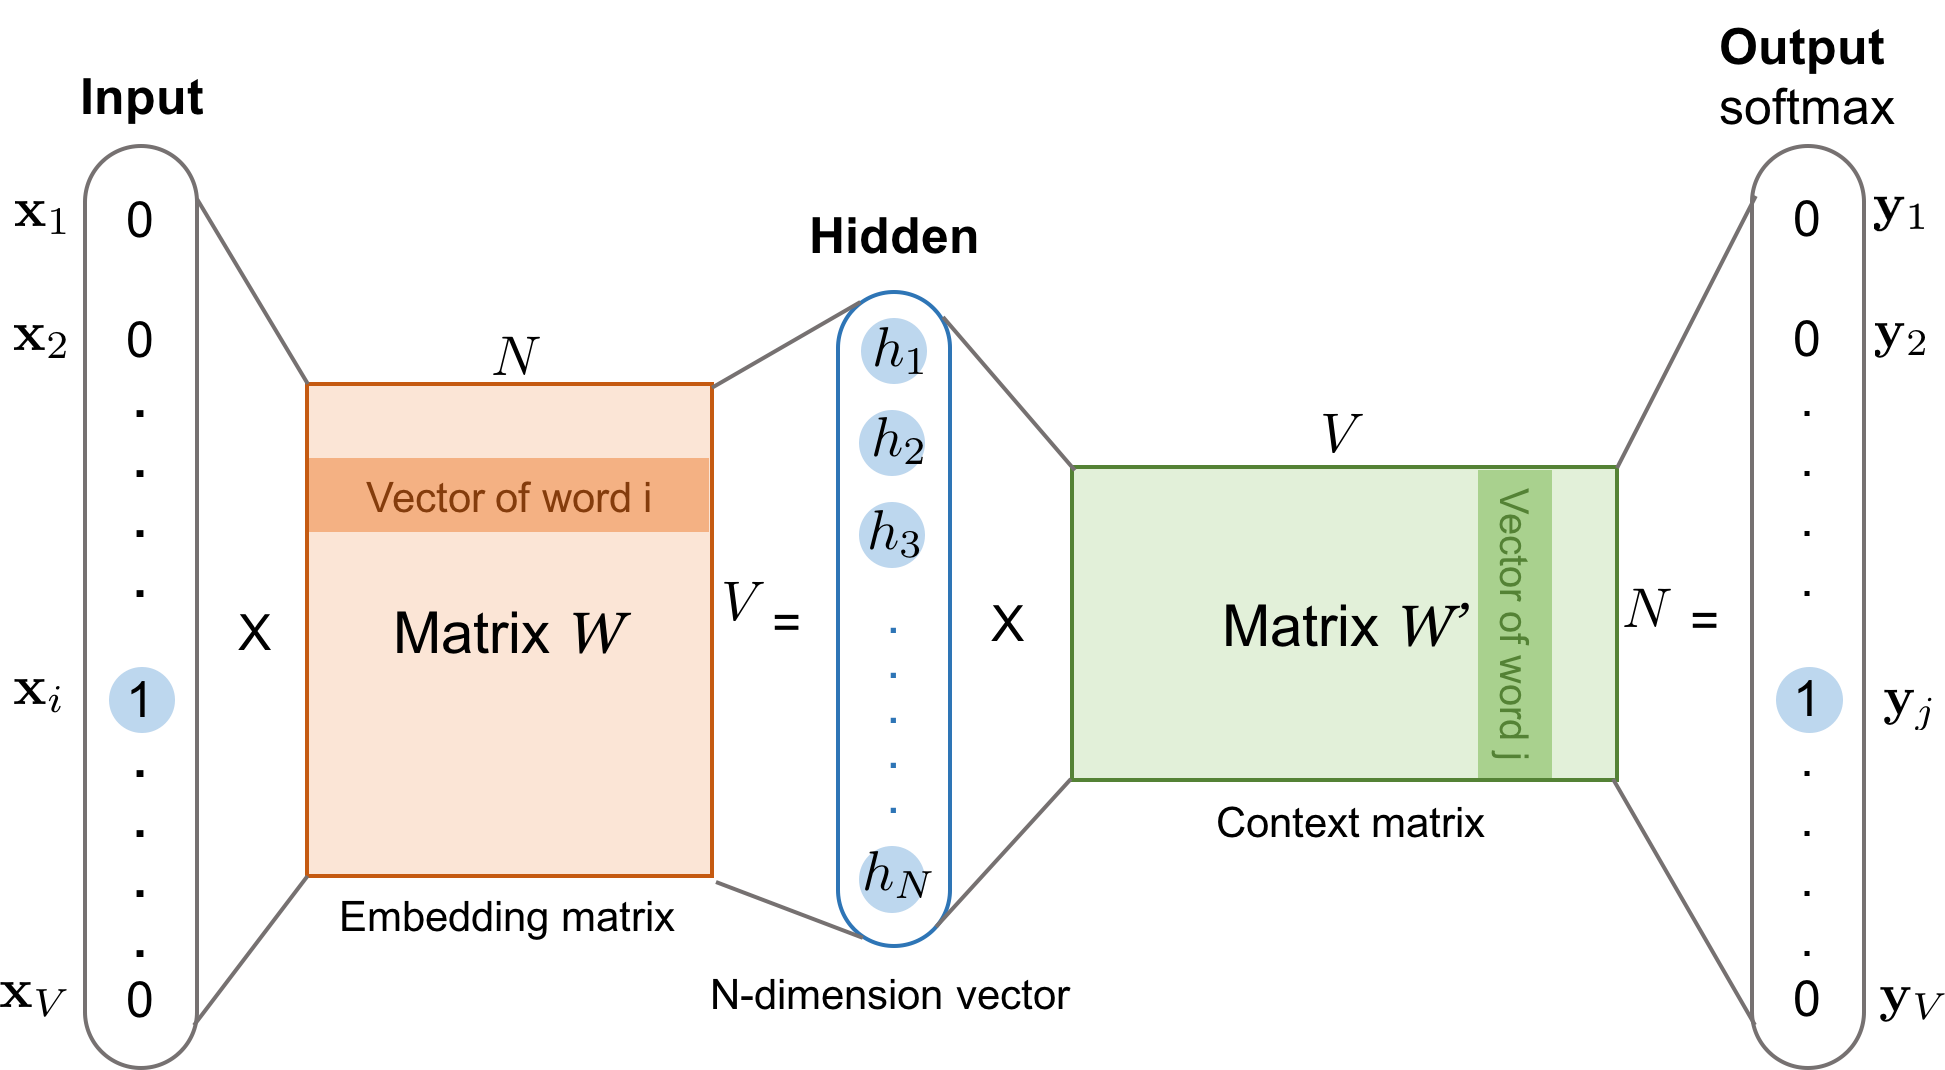
\includegraphics[scale=0.4]{../images/skip-gram.png}
    \caption[The Skip-gram Model]{The Skip-gram Model\protect\footnotemark}
	\label{fig:skip-gram}
\end{figure}

\footnotetext{Source: https://lilianweng.github.io/lil-log/2017/10/15/learning-word-embedding.html}

Since the softmax model requires a lot of computational space and time, we also use negative sampling with the Skip-gram model. Negative sampling will convert the multi-classification problem that the model is designed to solve into a binary-classification problem. First, the method will randomly select $K$ negative samples from the corpus that are irrelevant to the input word. $K$ is a hyper-parameter, usually between 5 and 20. The model will update $(K+1)\times N$ parameters using the sigmoid function, where $N$ is the dimension of the hidden layer $h$, and $+1$ accounts for the positive sample.

The probability that a word ($c$) appears within the context of the input word ($w$) can be defined as the following formula. The goal is to determine whether $c$ is in the context window of $w$ ($D=1$) or not ($D=0$) based on the input-context pairs $(w, c)$.

\begin{equation}
p(D=1 \mid w, c ; \theta)=\frac{1}{1+\exp \left(-\bar{c}_{\text {output }_{(j)}} \cdot w\right)} \in \mathbb{R}^{1}
\end{equation}

\subsection{Semantic Embedding}

We use gensim to implement Skip-gram with negative sampling from Word2Vec. We put the tokenized sentences generated by different tokenizers into gensim to train the general word embedding with semantics. The following are the main settings of the parameters: \textit{max\_vocab\_size} is 32000, \textit{vector\_size} is 300, \textit{epoch\_number} is 13, \textit{window\_size} is 5, the number of negative samples is 5, ignoring the words with total frequency lower than 5.

Some words may not be trained in the model, such as special tokens and low-frequency words. Therefore, the size of the trained embedding matrix and the tokenizer vocabulary is not identical, resulting in different coverage (Table~\ref{tab:semantic_coverage}). We calculate the mean and standard deviation of the whole embedding and randomly assign the empty word vectors using the normal distribution.

\vspace{0.5cm}
\begin{table}[h]
    \centering
    \begin{tabularx}{.9\textwidth}{ssss}\toprule
        Language & SentencePiece & Jieba & Janome \\\midrule
        Chinese & 95\% (30368/32000) & 93\% (29613/32000) & - \\
        Japanese & 97\% (30940/32000) & - & 93\% (29801/32000) \\
        \bottomrule
    \end{tabularx}
    \caption{The coverage of semantic embedding in vocabulary}
    \label{tab:semantic_coverage}
\end{table}

\subsection{Phonetic Embedding} \label{sec:phonetic_embedding}

The training method for phonetic embedding is mostly the same as semantic embedding. First, we convert tokenized sentences into phonetic encodings using the phonetic extraction techniques described in Section~\ref{sec:phonetic_data}. Second, we adopt the same training methods and parameters from semantic embedding. And last, we share the same vector of characters or words with the same pronunciation or spelling in the embedding matrix. Therefore, the coverage (Table~\ref{tab:phonetic_coverage}) will be even higher than the semantic embedding. The empty vectors are also randomly assigned using the normal distribution with mean and standard deviation from the whole embedding. 

\vspace{0.5cm}
\begin{table}[h]
    \centering
    \begin{tabularx}{.9\textwidth}{ssss}\toprule
        Language & SentencePiece & Jieba & Janome \\\midrule
        Chinese & 99\% (31753/32000) & 97\% (31068/32000) & - \\
        Japanese & 99\% (31698/32000) & - & 96\% (30809/32000) \\
        \bottomrule
    \end{tabularx}
    \caption{The coverage of phonetic embedding in vocabulary}
    \label{tab:phonetic_coverage}
\end{table}

\subsection{Joint Embedding} \label{sec:joint_embedding}

Several ways have been proposed to combine multiple embeddings, such as concatenation, training and blending separate embedding using the same model, and meta-embedding. Meta-embedding is a very vague term, but the core idea is to accept any kind of pre-trained embedding and fuse them into one (meta) embedding. Many studies on meta-embedding have been proposed \cite{kiela-etal-2018-dynamic, yin2015learning, muromagi2017linear}. The methods of meta-embedding can range from very complicated to very straightforward. This paper uses a simple averaging method \cite{coates-bollegala-2018-frustratingly} to merge semantic and phonetic embedding.

\section{Corpus Filtering} \label{sec:corpus_filtering}

We define custom rules and apply alignment scores from \textit{fast\_align} \cite{dyer2013simple} to perform corpus filtering to reduce noise, dataset size, and resource burden during training in the NMT system. The original dataset had 672,315 sentence pairs, which were reduced to 557,685 using rules and 462,582 using alignment scores.

\subsection{Pre-filtering rules}

We apply the following rules to exclude the pairs of sentences that do not match:

\begin{enumerate}
    \item Removing sentences that are too large in proportion to their length.
    \item Removing sentences that are too short or too long.
    \item Removing identical sentences.
    \item Removing sentences that cannot be correctly identified as Chinese or Japanese by the fastText identification model.
    \item Removing sentences with more English and numeric characters than Chinese and Japanese.
    \item Removing sentences that have more than one counterpart.
\end{enumerate}

\subsection{Scoring functions}

fast\_align is a tool based on \textit{IBM alignment model 2} for training statistical machine translation and alignment model. The score is the probability of the source sentence given the target sentence and its alignment. The algorithm iteratively estimates the probability of being each other translation for source-target pairs and optimal alignment given the word-to-word translation probabilities. 

In theory, the score should correlate with the degree of parallelism of the sentences. We remove the sentence pairs that are below a certain probability score threshold as shown in Table~\ref{tab:alignment_scores}. 

\newpage

\begin{table}[h]
    \centering
    \begin{tabularx}{.7\textwidth}{ss}\toprule
        Alignment Score Range & Number of sentence pairs \\\midrule
        $[-3, -81]$ & 173,100 \\
        $[-81, -160]$ & 287,882 \\\midrule
        $[-160, -238]$ & 93,134 \\
        $[-238, -317]$ & 3,540 \\
        $[-317, -395]$ & 29 \\
        \bottomrule
    \end{tabularx}
    \caption{Distribution of Sentence Pair Alignment Scores}
    \label{tab:alignment_scores}
\end{table}

We sampled some sentence pairs corresponding to alignment scores in Table~\ref{tab:alignment_samples}. The findings were that the lower the score, the longer the sentences tended to be, the more words were not translated, and the higher the proportion of proper nouns became.

\vspace{0.3cm}
\begin{table}[h]
    \centering
    \begin{CJK}{UTF8}{gbsn}
        \begin{tabularx}{\textwidth}{lb}\toprule
            Score & -52 \\
            {Chinese } & 残留性化学物质的物质循环模型的构建和再利用·废弃物政策评价的应用 \\
        \end{tabularx}
    \end{CJK}
    \begin{CJK}{UTF8}{long}
        \begin{tabularx}{\textwidth}{lb}
            Japanese & 残留性化学物質の物質循環モデルの構築とリサイクル・廃棄物政策評価への応用 \\
            \midrule
        \end{tabularx}
    \end{CJK}
    \begin{CJK}{UTF8}{gbsn}
        \begin{tabularx}{\textwidth}{lb}
            Score & -151 \\
            {Chinese } & 使用传统的轴组装工法的2层木制住宅,进行了室内甲醛浓度的测量,同时也研讨了上下楼层的甲醛浓度和换气量的关系。 \\
        \end{tabularx}
    \end{CJK}
    \begin{CJK}{UTF8}{long}
        \begin{tabularx}{\textwidth}{lb}
            Japanese & 在来軸組工法木造2階建住宅を用いて,室内ホルムアルデヒド濃度の測定を行うとともに,上下階のホルムアルデヒド濃度と換気量の関係も検討した。 \\
            \midrule
        \end{tabularx}
    \end{CJK}
    \begin{CJK}{UTF8}{gbsn}
        \begin{tabularx}{\textwidth}{lb}
            Score & -254 \\
            {Chinese } & 当我尽快编写了PID控制程序并运行后发现,不仅温度不能很好地稳定,还出现了“不规则振荡”现象(重复出现大幅度偏离控制值的振动),控制彻底失败了。 \\
        \end{tabularx}
    \end{CJK}
    \begin{CJK}{UTF8}{long}
        \begin{tabularx}{\textwidth}{lb}
            Japanese & 早速,PID制御のプログラムを書いて実行したところ,うまく温度が安定化しないどころかいわゆる“ハンチング”現象(制御値から大きく外れた振動を繰り返す)を起こしてしまい,見事,制御に失敗した \\
            \midrule
        \end{tabularx}
    \end{CJK}
    \begin{CJK}{UTF8}{gbsn}
        \begin{tabularx}{\textwidth}{lb}
            Score & -338 \\
            {Chinese } & ('关于葛根、黄苓、黄连汤之证,在『伤寒论』34条中叙述:“太阳病,桂枝证,医反下之,利遂不止,脉促者,表未解也,喘而汗出者,葛根黄芩黄连汤主之”。 \\
        \end{tabularx}
    \end{CJK}
    \begin{CJK}{UTF8}{long}
        \begin{tabularx}{\textwidth}{lb}
            Japanese & '葛根黄苓黄連湯証について,『傷寒論』34条に,「太陽病,桂枝の証,医反ってこれを下し,利遂に止まず,脈促のものは,表いまだ解せざるなり,ぜんして汗出づるものは,葛根黄苓黄連湯これを主る」という。 \\
            \midrule
        \end{tabularx}
    \end{CJK}
    \caption{Samples of Sentence Pairs with Alignment Scores}
    \label{tab:alignment_samples}
\end{table}

\section{NMT Model} \label{sec:nmt_model}

We will train and evaluate the NMT tasks in two classical models, the attention-based RNN model proposed by \cite{bahdanau2014neural}, and the Transformer model proposed by \cite{NIPS2017_3f5ee243}. We will explain the structure of models in this section. Furthermore, The use of parameters is presented in Section~\ref{sec:parameter}, the metric is explained in Section~\ref{sec:metric}, the results are listed in Section~\ref{sec:result}, and the case study is conducted in Section~\ref{sec:case_study}.

The two models and the following illustrative diagrams are derived from \textit{bentrevett/pytorch-seq2seq} \footnote{https://github.com/bentrevett/pytorch-seq2seq}. We utilize the source code and optimize the details, such as accelerating the decoding efficiency of the decoder.

\subsection{Attention-based GRU encoder-decoder Model} \label{sec:rnn}

This model (Seq2Seq) has three main components, namely Encoder, Attention, and Decoder. We used the \pythoninline{nn.Module} provided by PyTorch to implement three components and PyTorchLightning to combine and train the entire model.

\subsubsection{Encoder}

\begin{figure}[H]
	\centering
	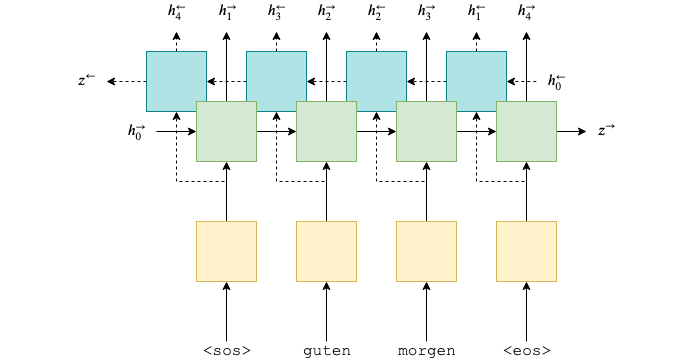
\includegraphics[scale=0.7]{../images/bi_encoder.png}
    \caption{The Encoder of Seq2Seq Model}
	\label{fig:seq2seq_encoder}
\end{figure}

The structure of the encoder (Figure~\ref{fig:seq2seq_encoder}) can be represented by the following equations. In eq. \ref{eq:eq1}, we enter the embedded tokens into the bi-directional GRU model to calculate the forward and backward hidden states $h$. 

\begin{equation}
    h_{\overrightarrow{t}} = \overrightarrow{\text{EncoderGRU}}(\text{emb}(x_{\overrightarrow{t}}), h_{\overrightarrow{t-1}}), 
    h_{\overleftarrow{t}} = \overleftarrow{\text{EncoderGRU}}(\text{emb}(x_{\overleftarrow{t}}), h_{\overleftarrow{t-1}})
    \label{eq:eq1}
\end{equation}

The output $H$ (in eq. \ref{eq:eq2}) represents the combination of hidden states in the last layer of the model and will be used to calculate the attention. 

\begin{equation}
    \text{outputs} (H) = \left\{h_1, h_2, \cdots, h_T\right\}, h_i = [h_{\overrightarrow{i}}; h_{\overleftarrow{i}}] \text{ for } i \in \{1,\cdots T\}
    \label{eq:eq2}
\end{equation}

The obtained hidden states $\overrightarrow{z}$ and $\overleftarrow{z}$ (in eq. \ref{eq:eq3}) will be used as the initial hidden states of the decoder. 

\begin{equation}
    \overrightarrow{z} = h_{\overrightarrow{T}},
    \overleftarrow{z} = h_{\overleftarrow{T}}
    \label{eq:eq3}
\end{equation}

Since the decoder is not bidirectional, we enter the hidden states $\overrightarrow{z}$ and $\overleftarrow{z}$ into a linear layer $g$ and a activation function $tanh$ (in eq. \ref{eq:eq4}) to get the condensed context vector $z$, also called $s_0$.

\begin{equation}
    z = \tanh(g(\text{cat}(\overrightarrow{z}, \overleftarrow{z}))) = s_0
    \label{eq:eq4}
\end{equation}

\subsubsection{Attention}

\begin{figure}[h]
	\centering
	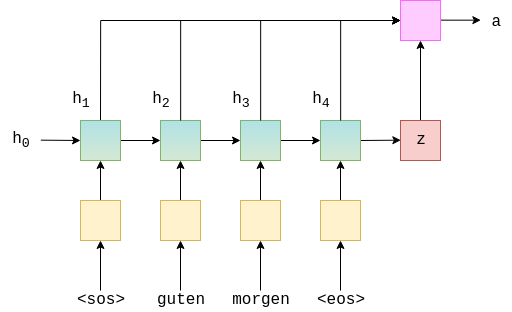
\includegraphics[scale=0.7]{../images/seq2seq_encoder_attention.png}
    \caption{The Attention of Seq2Seq Model}
	\label{fig:seq2seq_attention}
\end{figure}

The attention layer (Figure~\ref{fig:seq2seq_attention}) generates an array of the same length as the source sentence, representing how much attention was given to each token in the source sentence when predicting the next token $\hat{y}_{t+1}$. The attention layer is a linear layer, and each time it takes the previous hidden state $s_{t-1}$ of the decoder (the first time is the $z$ or $s_0$ from encoder), and the output $H$ from encoder to compute an energy value $E_t$ with $tanh$ activation function (in eq. \ref{eq:eq5}).

\begin{equation}
    E_t = \tanh(\text{attn}(s_{t-1}, H)) \label{eq:eq5}
\end{equation}

Because the shape of the energy value $E_t$ is (\textit{src\_len} \footnote{The length of source sentence}, \textit{hid\_dim} \footnote{The dimension of hidden layer}), it will enter into a linear layer $v$ with the shape (\textit{hid\_dim}, 1) (in eq. \ref{eq:eq6}) to get the attention sequence $\hat{a}_t$ with the shape (\textit{src\_len}). The parameters learned in the linear layer $v$ can be imagined as the weight of the energy value $E_t$ for each token in the source sentence.

\begin{equation}
     \hat{a}_t = v(E_t) \label{eq:eq6}
\end{equation}

The attention sequence $\hat{a}_t$ will be passed to the softmax layer (in eq. \ref{eq:eq7}) so that all the attention values add up to 1. The process combines with the mask to zero out the attention of the [PAD] tokens. 

\begin{equation}
a_t = \text{softmax}(\hat{a}_t) \label{eq:eq7}
\end{equation}

\subsubsection{Decoder}

\begin{figure}[h]
	\centering
	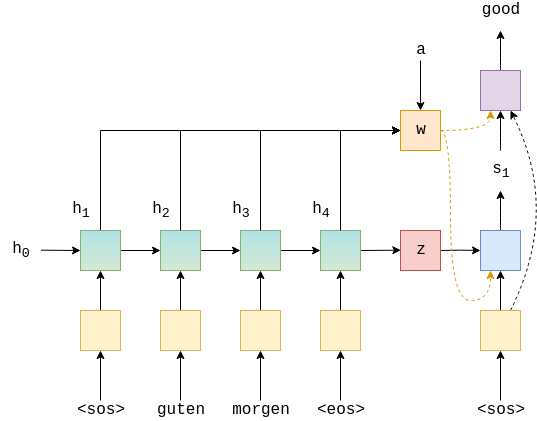
\includegraphics[scale=0.7]{../images/seq2seq_decoder_attention.png}
    \caption{The Decoder of Seq2Seq Model}
	\label{fig:seq2seq_decoder}
\end{figure}

The decoder (Figure~\ref{fig:seq2seq_decoder}) first uses the previous hidden state $s_{t-1}$ and the encoder output $H$ to compute the attention vector $a_t$ for the current time-step $t$. The attention vector $a_t$ will perform a matrix multiplication with $H$ (in eq. \ref{eq:eq8}) to produce the weighted sum $w_t$ that represents the attention to each token in the source sentence.

\begin{equation}
    w_t = a_tH \label{eq:eq8}
\end{equation}

The decoder then takes the embedded target token $d(y_t)$, the weighted source vector $w_t$, and the previous hidden state $s_{t-1}$ into the one-directional GRU model to compute the current hidden state $s_t$ (in eq. \ref{eq:eq9}).

\begin{equation}
    s_t = \text{DecoderGRU}(d(y_t), w_t, s_{t-1}) \label{eq:eq9}
\end{equation}

Finally, the decoder uses $d(y_t)$, $w_t$, $s_t$ and a linear layer $f$ to predict the next token $\hat{y}_{t+1}$ (in eq. \ref{eq:eq10}). We will apply the teacher forcing technique, which has a 0.5\% chance of using the predicted token and a 0.5\% chance of using the ground truth token as the next target input token.

\begin{equation}
    \hat{y}_{t+1} = f(d(y_t), w_t, s_t) \label{eq:eq10}
\end{equation}

\subsection{Transformer} \label{sec:transformer}

The Transformer is an attention-driven model that uses the attention mechanism to process data in either encoder or decoder. We first describe the attention mechanism and then introduce it to the encoder and decoder.

\subsubsection{Attention}

\begin{figure}[h]
    \centering
    \begin{subfigure}[b]{0.45\textwidth}
        \centering
        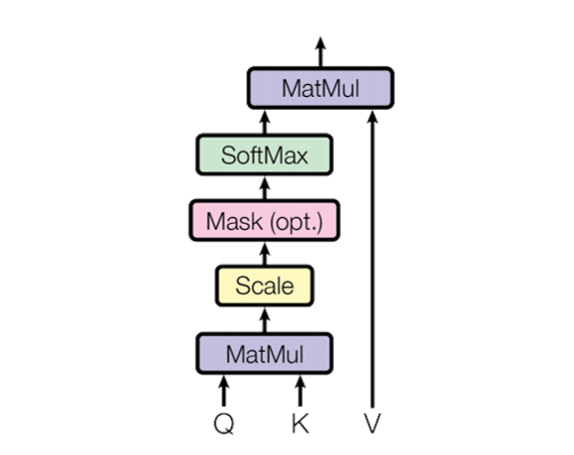
\includegraphics[width=\textwidth]{../images/transformer-attention.png}
        \caption{Scaled Dot-Product Attention}
        \label{fig:transformer_attention1}
    \end{subfigure}
    \hfill
    \begin{subfigure}[b]{0.45\textwidth}
        \centering
        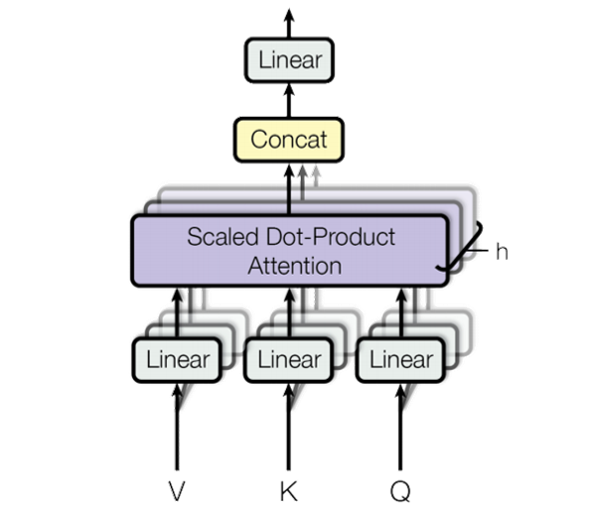
\includegraphics[width=\textwidth]{../images/transformer-multihead-attention.png}
        \caption{Multi-Head Attention}
        \label{fig:transformer_attention2}
    \end{subfigure}

    \caption{The Multi-head Attention of Tranformer}
	\label{fig:transformer_attention}
\end{figure}

In the Transformer, Attention layer requires three elements, namely query ($Q$), key ($K$), and value ($V$), as shown in Figure~\ref{fig:transformer_attention1}. To begin with, the energy value is generated by taking the dot product between query $Q$ and key $K$. It is then scaling by the square root of \textit{head\_dim} \footnote{The hidden state dimension of each head in Multi-Head Attention} ($\sqrt{d_k}$) to avoid gradient vanishing. After that, the energy value is fed into the softmax layer to get the attention sequence and finally multiplied with the value $V$ to get the weighted sum (in eq. \ref{eq:eq11}).

\begin{equation}
\text{Attention}(Q, K, V) = \text{Softmax}\left(\frac{QK^T}{\sqrt{d_k}}\right)V \label{eq:eq11}
\end{equation}

The Transformer model splits query $Q$, key $K$, and value $V$ into multiple heads with smaller dimensions and trains them separately (Figure~\ref{fig:transformer_attention2}). They are divided into heads by the linear layers ($W_i^Q, W_i^K, W_i^V$). Each has the size that equals the dimension of the hidden state divided by the number of heads. 

\begin{equation}
\text{head}_i = \text{Attention}(QW_i^Q, KW_i^K, VW_i^V) \label{eq:eq12}
\end{equation}

After all the heads pass through the attention layer (in eq \ref{eq:eq12}), they are re-concatenated and pass through the last linear layer $W^O$ to get the final weighted sum (in eq \ref{eq:eq13}).

\begin{equation}
\text{MultiHeadAttention}(Q, K, V) = \text{Concat}(\text{head}_1, \cdots, \text{head}_h)W^O
\label{eq:eq13}
\end{equation}

\subsubsection{Encoder and Encoder Layers}

\begin{figure}[h]
	\centering
	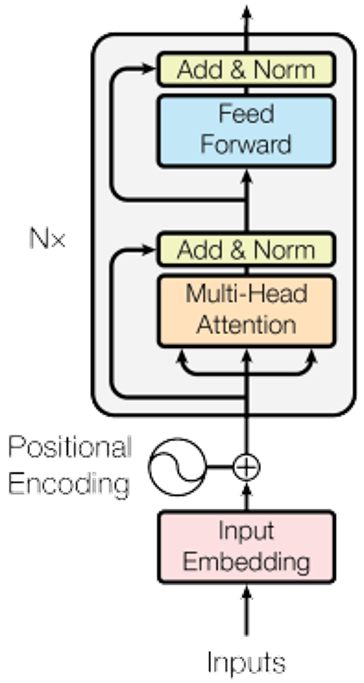
\includegraphics[scale=0.7]{../images/transformer-encoder.png}
    \caption{The Encoder of Transformer}
	\label{fig:transformer_encoder}
\end{figure}

Unlike the RNN model, the input tokens will generate the corresponding number of context vectors directly after passing through the encoder. For example, if the input has 5 tokens $X = (x_1, x_2, x_3, x_4, x_5)$, the encoder will generate 5 context vectors $Z = (z_1, z_2, z_3, z_4, z_5)$ for the decoder to predict.

The tokens are passed to the word embedding and retrieved the position information by the positional embedding. The size of the positional embedding is equal to the length of the sentence; if the sentence length is 100, then the size of the positional embedding will be 100. The word embedding is added to the positional embedding to obtain the text and position information. However, the word embedding is multiplied by a scaling factor $\sqrt{d_\text{model}}$, which is used to reduce the variance of the embedding.

An encoder will have multiple encoder layers. Each of them contains an attention layer and a position-wise feedforward layer (which can be considered as a large linear layer). In addition to these two components, there are also residual connection and layer normalization, which aim to generalize all parameters and prevent gradients from disappearing, making it easier to train networks with a large number of parameters. Because the attention is calculated from the source sentence and itself, it is also called self-attention. 

\subsubsection{Decoder and Decoder Layers}

\begin{figure}[h]
	\centering
	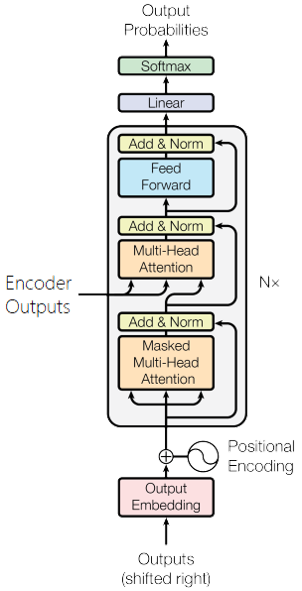
\includegraphics{../images/transformer-decoder.png}
    \caption{The Decoder of Transformer}
	\label{fig:transformer_decoder}
\end{figure}

The architecture of the decoder is almost identical to that of the encoder. The decoder feeds the embedded-target-tokens into several decoder layers, and predicts the next target token $\hat{y}$ with source context vector $Z$. Following this, it computes the loss by the predict token $\hat{y}$ and the answer token $y$, and updates all the weights of the network.

There are three main components in a decoder layer. First, the decoder has a masked multi-head attention layer, in which the target sentence will perform self-attention with itself and a special mask to prevent the decoder from seeing the future words in advance. Second, the multi-head attention layer is calculated with the context vector from the masked multi-head attention layer as the query $Q$ and the encoder context vector as the key $K$ and value $V$. Third, the last position-wise feedforward layer receives the results of the previous layer and outputs the final context vector to predict the next token $\hat{y}$.

\section{Embedding Analysis} \label{sec:embedding_analysis}

We will examine the effectiveness of joint semantic-phonetic embedding using four methods implemented in gensim. We expect joint semantic-phonetic embedding to retain the word similarity, analogical reasoning, and outlier detection capabilities that semantic embedding possesses. We are also interested in whether the joint embedding can enhance the impact on homonyms and heteronyms. All examination findings will be discussed in Section~\ref{sec:analysis}.

% 講解這個東西在幹嘛的。怎麼算。怎麼用 gensim 跑。

\subsection{Word Similarity} \label{sec:similarity}

The purpose of word similarity is to evaluate the closeness and relatedness of any two words in the given embedding. This paper measures the word similarity by calculating the cosine distance, which is equal to 1 - cosine similarity; the higher the similarity, the shorter the distance. The cosine similarity estimates the relatedness between two vectors by measuring the cosine of the angle between them (in eq. \ref{eq:eq14}). The cosine similarity of two vectors with the same direction is 1, the angle of 90° is 0, and the opposite direction is -1.

\begin{equation}
    \text { similarity }=\cos (\theta)=\frac{A \cdot B}{\|A\|\|B\|}=\frac{\sum_{i=1}^{n} A_{i} \times B_{i}}{\sqrt{\sum_{i=1}^{n}\left(A_{i}\right)^{2}} \times \sqrt{\sum_{i=1}^{n}\left(B_{i}\right)^{2}}} \label{eq:eq14}
\end{equation}

This paper uses similarity distance to compare the distance of synonyms under different embeddings to examine whether joint embedding can preserve the semantic properties.

\subsection{Analogical Reasoning} \label{sec:analogy}

Analogical reasoning is to evaluate the ability of embeddings to apply arithmetic operations to reasoning. Given a set of three words, $a$, $a*$ and $b$, the task requires identifying the word $b*$, i.e., the relation $b$:$b*$ is the same as the relation $a$:$a*$. For example, when $a=\text{Tokyo}$, $a*=\text{Japan}$, $b=\text{Taipei}$, the embedding need to be able to predict $b*=\text{Taiwan}$. The analogical reasoning can be shown as the following eq. \ref{eq:eq15}.

\begin{equation}
    a - a* + b = b* \label{eq:eq15}
\end{equation}

\subsection{Outlier Detection} \label{sec:outlier}

Outlier Detection tests the ability of embeddings to perform the task of word categorization. The embeddings are required to identify the semantically anomalous word from a defined word cluster. For example, when the word cluster contains ``apple, bird, cat, dog'', the embedding needs to predict the target word as ``apple''.

\subsection{Homonym and Heteronym} \label{sec:homonym_heteronym}

This task is an extension of word similarity tasks. We expect the joint embedding with additional phonetic information reduces the impact of possible noise on the NMT system (i.e. the impact of homonyms). Homonyms refer to the words that have the same pronunciation and spelling but different meanings. The evaluation method is to ensure that the distance between homonyms is as short as possible. At the same time, we expect that phonetic information will help the joint embedding to increase the distance between heteronyms. Heteronyms refer to words that have identical writing but different pronunciation, spelling, and meaning. Increasing the distance between heteronyms means strengthening the semantics between words.
